\chapter{Singular Perturbation} \label{chap:singular-perturbation}
When dealing with the accelerating velocity profile, spectral methods struggle to yield meaningful results because of the singularity at the nozzle throat ($z=0$). This chapter is dedicated to analyze the polynomial eigenvalue problem with accelerating velocity profile. We start by showing the existence of the singularity of Eq.~(\ref{eq:polynomial-eigenvalue-problem}), and how spectral methods introduced in previous chapter failed to resolve solutions. Then we will discuss the concept of singular perturbation and will pick up regular solutions to Eq.~(\ref{eq:polynomial-eigenvalue-problem}) near the nozzle throat $z=0$ using Frobenius method. Finally, we will introduce shooting method and use it together with the regular solutions to find eigenmodes.

\section{Presence of Singularity in Transonic Cases} \label{sec:presence-of-singularity}
In order to see the existence of the singularity, we rearrange the terms the polynomial eigenvalue problem, Eq.~(\ref{eq:polynomial-eigenvalue-problem}),
\begin{equation} \label{eq:singular-perturbation-problem}
	\begin{aligned}
		  & (1-v_0^2)\pdv[2]{\tilde{v}}{z}                                                                                                                                        \\
		+ & \left[2i\omega v_0 - \left(3v_0 + \frac{1}{v_0}\right)\pdv{v_0}{z}\right]\pdv{\tilde{v}}{z}                                                                           \\
		+ & \left[\omega^2 + 2i\omega\pdv{v_0}{z} -\left(1 - \frac{1}{v_0^2}\right)\left(\pdv{v_0}{z}\right)^2 - \left(v_0 + \frac{1}{v_0}\right)\pdv[2]{v_0}{z} \right]\tilde{v} \\
		= & 0.
	\end{aligned}
\end{equation}
This is a second order ordinary differential equation defined on region $[-1,1]$.

For transonic (accelerating and decelerating) velocity profiles (Fig.~\ref{fig:velocity-profiles}), the plasma flow is at sonic point at the throat of the nozzle, $v_0(0)=1$. Therefore, the highest order term vanishes at $z=0$. It is a singular point, and it is the  cause of the failure of spectral method, see Fig.~(\ref{fig:failure-of-spectral-method}). Spectral method is unable to resolve meaningful eigenfunctions, the eigenfunctions are squeezed together at $z=0$, hence resulting in wrong eigenvalues.

\begin{figure} [htbp]
	\centering
	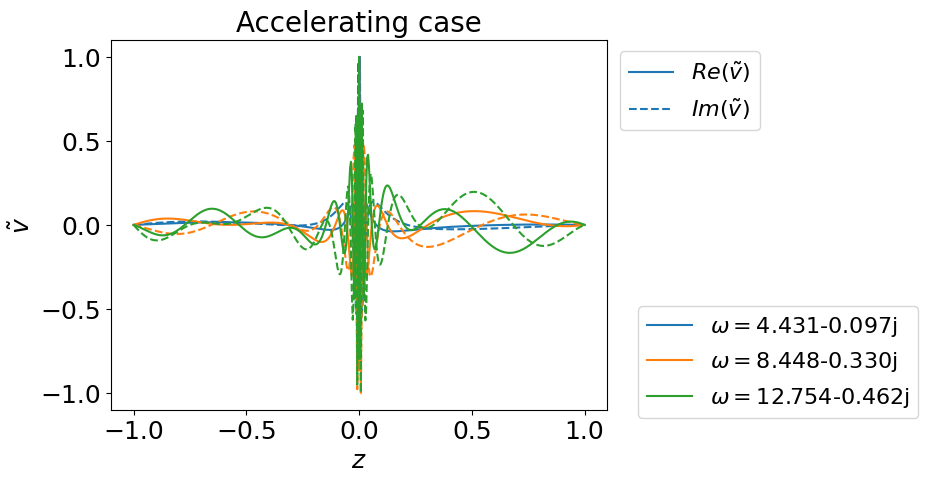
\includegraphics[width=0.7\textwidth]{figures/results-bad-accelerating-v}
	\caption{An attempt to solve the polynomial eigenvalue problem, Eq.~(\ref{eq:polynomial-eigenvalue-problem}) using finite-difference. Eigenfunctions are squeezed to the center of the nozzle due to the existence of the singularity at $z=0$.}
	\label{fig:failure-of-spectral-method}
\end{figure}

\section{Expansion at Singularity}
In this section, we will try to extract the regular solutions to Eq.~(\ref{eq:singular-perturbation-problem}) using Frobenius method. It is speculated such regular solutions exist. Further analysis and numerical simulations also validate the existence of such solutions. In order to find them, we need to expand terms in Eq.~(\ref{eq:singular-perturbation-problem}) about the singularity.

The first task is to linearize the terms with $v_0$ about the singularity. The linearization of $v_0(z) = 1 + v_0'(0)z$ is a good approximation to the original function $v_0(z)$ because the transonic velocity profiles are linear in the neighborhood of $z=0$, as we can see from Fig.~\ref{fig:velocity-profiles}. Therefore, through some simple algebra we obtain,
\begin{equation}
	\begin{aligned}
		1-v_0^2              & = -2v_0'(0)z    \\
		3v_0 + \frac{1}{v_0} & = 4 + 2v_0'(0)z \\
		1-\frac{1}{v_0^2}    & = 2v_0'(0)z     \\
		v_0 + \frac{1}{v_0}  & = 2.
	\end{aligned}
\end{equation}

Then Eq.~(\ref{eq:singular-perturbation-problem}) becomes
\begin{equation} \label{eq:perturbed-equation-full}
	\begin{aligned}
		- & 2v_0'(0)z\pdv[2]{\tilde{v}}{z}                                              \\
		+ & [2i\omega - 4v_0'(0) + (2i\omega - 2v_0'(0))z]\pdv{\tilde{v}}{z}            \\
		+ & \left[\omega^2 + 2i\omega v_0'(0) - 2v_0''(0) - 2v_0'(0)^3z\right]\tilde{v}
		= 0.
	\end{aligned}
\end{equation}

In fact, we can further simply the equation by dropping all $z$ terms except the first term (second-order derivative term). It can be shown that dropping the $z$ terms except the second derivative in Eq.~(\ref{eq:perturbed-equation-full}) does not affect the first order correction ($\tilde{v}$ is the same up to $z$ term), it is an acceptable approximation.
\begin{equation}
	- 2v_0'(0)z\pdv[2]{\tilde{v}}{z}
	+ (2i\omega - 4v_0'(0))\pdv{\tilde{v}}{z}
	+ (\omega^2 + 2i\omega v_0'(0) - 2v_0''(0))\tilde{v}
	= 0.
\end{equation}

Dividing by the first coefficient, we have
\begin{equation}
	z\pdv[2]{\tilde{v}}{z} + a\pdv{\tilde{v}}{z} + b\tilde{v} = 0,
	\label{eq:perturbed-equation}
\end{equation}
where
\begin{equation}
	a = \frac{2i\omega - 4v_0'(0)}{-2v_0'(0)}; \quad
	b = \frac{\omega^2 + 2i\omega v_0'(0) - 2v_0''(0)}{-2v_0'(0)}.
\end{equation}

Use Frobenius method, we assume the velocity perturbation can be written as a power series in $z$,  $\tilde{v} = \sum_{n\geq 0}c_nz^{n+r}$. By substituting the power series into Eq.~(\ref{eq:perturbed-equation}) we have
\begin{equation}
	\sum_{n \geq 0} (n+r)(n+r+1) c_n z^{n+r-1} + a(n+r)c_nz^{n+r-1} + bc_nz^{n+r} = 0.
\end{equation}
Shift the power of the last term we get
\begin{equation}
	\sum_{n \geq 0} (n+r)(n+r+1) c_n z^{n+r-1} + a(n+r)c_nz^{n+r-1} + \sum_{n \geq 1} bc_{n-1}z^{n+r-1} = 0.
\end{equation}

Setting $n=0$, we get the indicial equation
\begin{equation}
	c_0 r(r-1) + c_0 ar = 0 \Rightarrow c_0r(r+a-1) = 0.
\end{equation}
We get two different roots, $r=0$ and $r=1-a$. They correspond to finite solution and diverging solution near the singularity, respectively.

The coefficients are given by recurrence relation
\begin{equation}
	(n+r)(n+r-1)c_n + a(n+r)c_n + bc_{n-1} = 0
	\Rightarrow
	c_n = \frac{-bc_{n-1}}{(n+r)(n+r-1+a)}.
\end{equation}
Solving this relation we get explicit expression for $c_n$, $n\in\mathbb{N}$,
\begin{equation}
	\begin{aligned}
		c_n & = \frac{(-1)^n b^n c_0}{\prod_{k=0}^{n-1} (n+r-k)(n+r-1+a-k)}               \\
		    & = (-1)^n b^n c_0 \frac{\Gamma(r+1)\Gamma(r+a)}{\Gamma(n+r+1)\Gamma(n+r+a)},
	\end{aligned}
	\label{eq:coefficient}
\end{equation}
where $\Gamma$ is the Gamma function. Therefore, we successfully extracted the regular solution (corresponding to the root $r=0$) in the form of power series,
\begin{equation} \label{eq:regular-solution}
	\begin{aligned}
		\tilde{v} & = c_0 + c_1z + c_2z^2 + \cdots                                \\
		          & = c_0 - c_0\frac{b}{a}z + c_0\frac{b^2}{2a(1+a)}z^2 + \cdots.
	\end{aligned}
\end{equation}

It is worth to mention that the diverging solution (corresponding to the root $r=a$) goes like
\begin{equation}
	\tilde{v}(z) \sim z^{1-a} = z^{-1-\omega_i/v_0'(0)}z^{i\omega_r/v_0'(0)},
\end{equation}
where $\omega = \omega_r + i\omega_i$. Meaning that the divergent solution will start to diverge when $\omega_i > -v'(0)$.

\section{Shooting Method}
The existence of divergent solutions makes the problem hard to solve numerically using spectral method. One workaround involves manually selecting regular solutions during the numerical process. The shooting method, a suitable numerical technique, is capable of incorporating information of regular solutions. In other words, $\tilde{v}$ and its derivatives at the nozzle throat $z=0$ can be incorporate into the numerical process. Due to this restriction of singularity, we are not allowed to impose any boundary condition at the nozzle exit, $z=1$, anymore because the information of the regular solution already serve as a boundary condition.

Our polynomial eigenvalue problem, Eq.~(\ref{eq:polynomial-eigenvalue-problem}), can be formulated in the following form,
\begin{equation}
	f(z, \tilde{v}, \tilde{v}', \tilde{v}''; \omega) = 0
	\quad
	-1\leq z \leq 0,
	\quad
	\tilde{v}(-1) = 0, \tilde{v}(0) = 1,
\end{equation}
where $f$ is the function defined on the left of equal sign of Eq.~(\ref{eq:polynomial-eigenvalue-problem}). The task for shooting method is to find eigenvalues $\omega$ and their corresponding eigenfunctions $\tilde{v}$ such that $f=0$ holds. Meanwhile, the eigenfunctions must satisfy the boundary conditions at the entrance $z=-1$ and at the throat $z=0$. After obtaining the solutions, we can extend the solution to $z=1$. The extension is unique, more details will be explained later.

However, to make the formulation more suitable for numerical computation, we would like to rewrite the second differential equation as two first order differential equations,
\begin{equation}
	\dv{z}\mathbf{\tilde{u}} = \mathbf{f}(\mathbf{\tilde{u}},z;\omega),
	\quad
	-1 \leq z \leq 0,
	\quad
	\tilde{v}(-1) = 0, \tilde{v}(0) = 1.
	\label{eq:shooting-method-formulation}
\end{equation}
Let $\mathbf{\tilde{u}} = [\tilde{v}, \tilde{u}]^T$, the polynomial eigenvalue problem is transformed to
\begin{align*}
	\tilde{v}' & = \tilde{u}                \\
	\tilde{u}' & = \frac{-1}{1-v_0^2}\left[
		\omega^2\tilde{v} + 2i\omega(v_0+v_0'\tilde{v}) - \left(3v_0 - \frac{1}{v_0}\right)v_0'\tilde{u} - \left(1-\frac{1}{v_0}^2\right)(v_0')^2\tilde{v} - \left(v_0+\frac{1}{v_0}v_0''\tilde{v}\right)
		\right].
\end{align*}
Together with two boundary conditions, $\tilde{v}(-1) = 0$ and $\tilde{v}(0) = 1$. The task of shooting method remains the same: find $\mathbf{\tilde{u}}$ and $\omega$ such that $\dv*{\mathbf{\tilde{u}}}{z} = \mathbf{f}$ and $\tilde{v}$ must satisfy the boundary conditions.

Suppose $\omega$ is given. We can find $\mathbf{\tilde{u}}(-1)$ by solving the following I.V.P. with initial conditions at $z=0$, and hence $\tilde{v}(-1)$ by applying 4th order Runge-Kutta method (RK4) to the following IVP,
\begin{equation}
	\dv{z}\mathbf{\tilde{u}} = \mathbf{f}(\mathbf{\tilde{u}},z;\omega), \quad
	-1 \leq z \leq 0, \quad
	\mathbf{\tilde{u}}(0)=\mqty[\tilde{v}(0) \\ \tilde{u}(0)], \dv{z}\mathbf{\tilde{u}}(0) =\mqty[\tilde{v}'(0) \\ \tilde{u}'(0)].
	\label{eq:shooting-method-ivp}
\end{equation}
The information of the regular solution is built into the numerical process by setting the initial conditions,
\begin{equation}
	\begin{aligned}
		\mathbf{\tilde{u}}       & = \mqty[\tilde{v}(0)  \\ \tilde{u}(0)]
		= \mqty[c_0                                      \\ c_1]
		= \mqty[1                                        \\ (2i\omega v_0'-2v_0'')/2v_0'] \\
		\dv{z}\mathbf{\tilde{u}} & = \mqty[\tilde{v}'(0) \\ \tilde{u}'(0)]
		= \mqty[\tilde{u}(0)                             \\ c_2]
		= \mqty[(2i\omega v_0'-2v_0'')/2v_0'             \\ -((v_0')^4+(2i\omega v_0' + (v_0')^2 - v_0'')(i\omega v_0' - v_0''))/(v_0'(2i\omega-6v_0'))].
	\end{aligned}
\end{equation}
The coefficients $c_0, c_1$, and $c_2$ are obtained from the power series expansion of $\tilde{v}$ near $z=0$, Eq.~(\ref{eq:regular-solution}).

The above step can be abstracted as a function, $h(\omega) = \tilde{v}(-1)$. This function takes in a variable $\omega$, and it outputs the value $\tilde{v}(-1)$ by applying RK4 to the I.V.P. Eq.~(\ref{eq:shooting-method-ivp}). We then apply root finding algorithm to this function $h$ to find $\omega$ such that $\tilde{v}$ satisfies the boundary condition at the entrance, $h(\omega)=\tilde{v}(-1)=0$. This process can be viewed as trying to land a projectile at certain location, i.e., $\tilde{v}(-1)=0$, by adjusting the shooting angle, i.e., $\omega$, hence the name shooting method.

After finding $\omega$, we can extend the numerical solution $\tilde{v}$ to the region $[0,1]$. We simply apply RK4 to the following I.V.P.
\begin{equation}
	\dv{z}\mathbf{\tilde{u}} = \mathbf{f}(\mathbf{\tilde{u}},z;\omega), \quad
	0 \leq z \leq 1, \quad
	\mathbf{\tilde{u}}(0)=\mqty[\tilde{v}(0) \\ \tilde{u}(0)], \dv{z}\mathbf{\tilde{u}}(0) =\mqty[\tilde{v}'(0) \\ \tilde{u}'(0)].
\end{equation}
Since $\omega$ is already found, the initial conditions are given. The function $\mathbf{f}$ is continuous in $z$ on $[0,1]$ and is Lipschitz in $\mathbf{\tilde{u}}$ due to the fact that $\mathbf{f}$ is continuous on a compact region $[0,1]$. Hence, the solution to this I.V.P. exists and is unique.


\section{Plasma Flow with Accelerating Velocity Profile}
Starting from the singular point, we shoot the regular solution to the left boundary. We find the set of eigenvalues such that $\tilde{v}(-1)=0$. With these eigenvalues, we can extend the solution to the supersonic region $(0,1]$. The first few eigenmodes are drawn in Fig.~\ref{fig:results-accelerating-v}. The eigenmodes indicates that the accelerating plasma flow is stable.
\begin{figure} [H]
	\centering
	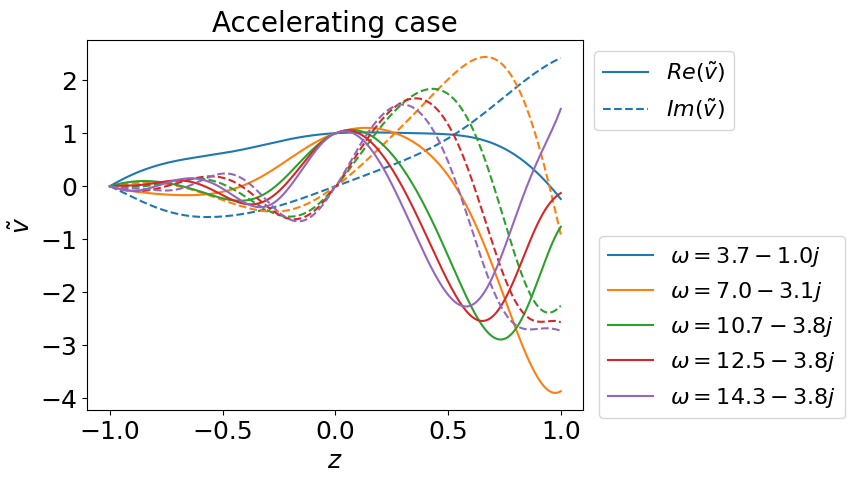
\includegraphics[width=0.7\linewidth]{figures/results-accelerating-v}
	\caption{Showing the first 5 eigenmodes, they are stable.}
	\label{fig:results-accelerating-v}
\end{figure}
